\section{Exercise 2: Vandermonde matrix}

\noindent The code:

\lstinputlisting{vandermonde.py}

\noindent The output:

\input{vandermonde_output.txt}

\begin{figure}[H]
    \centering
    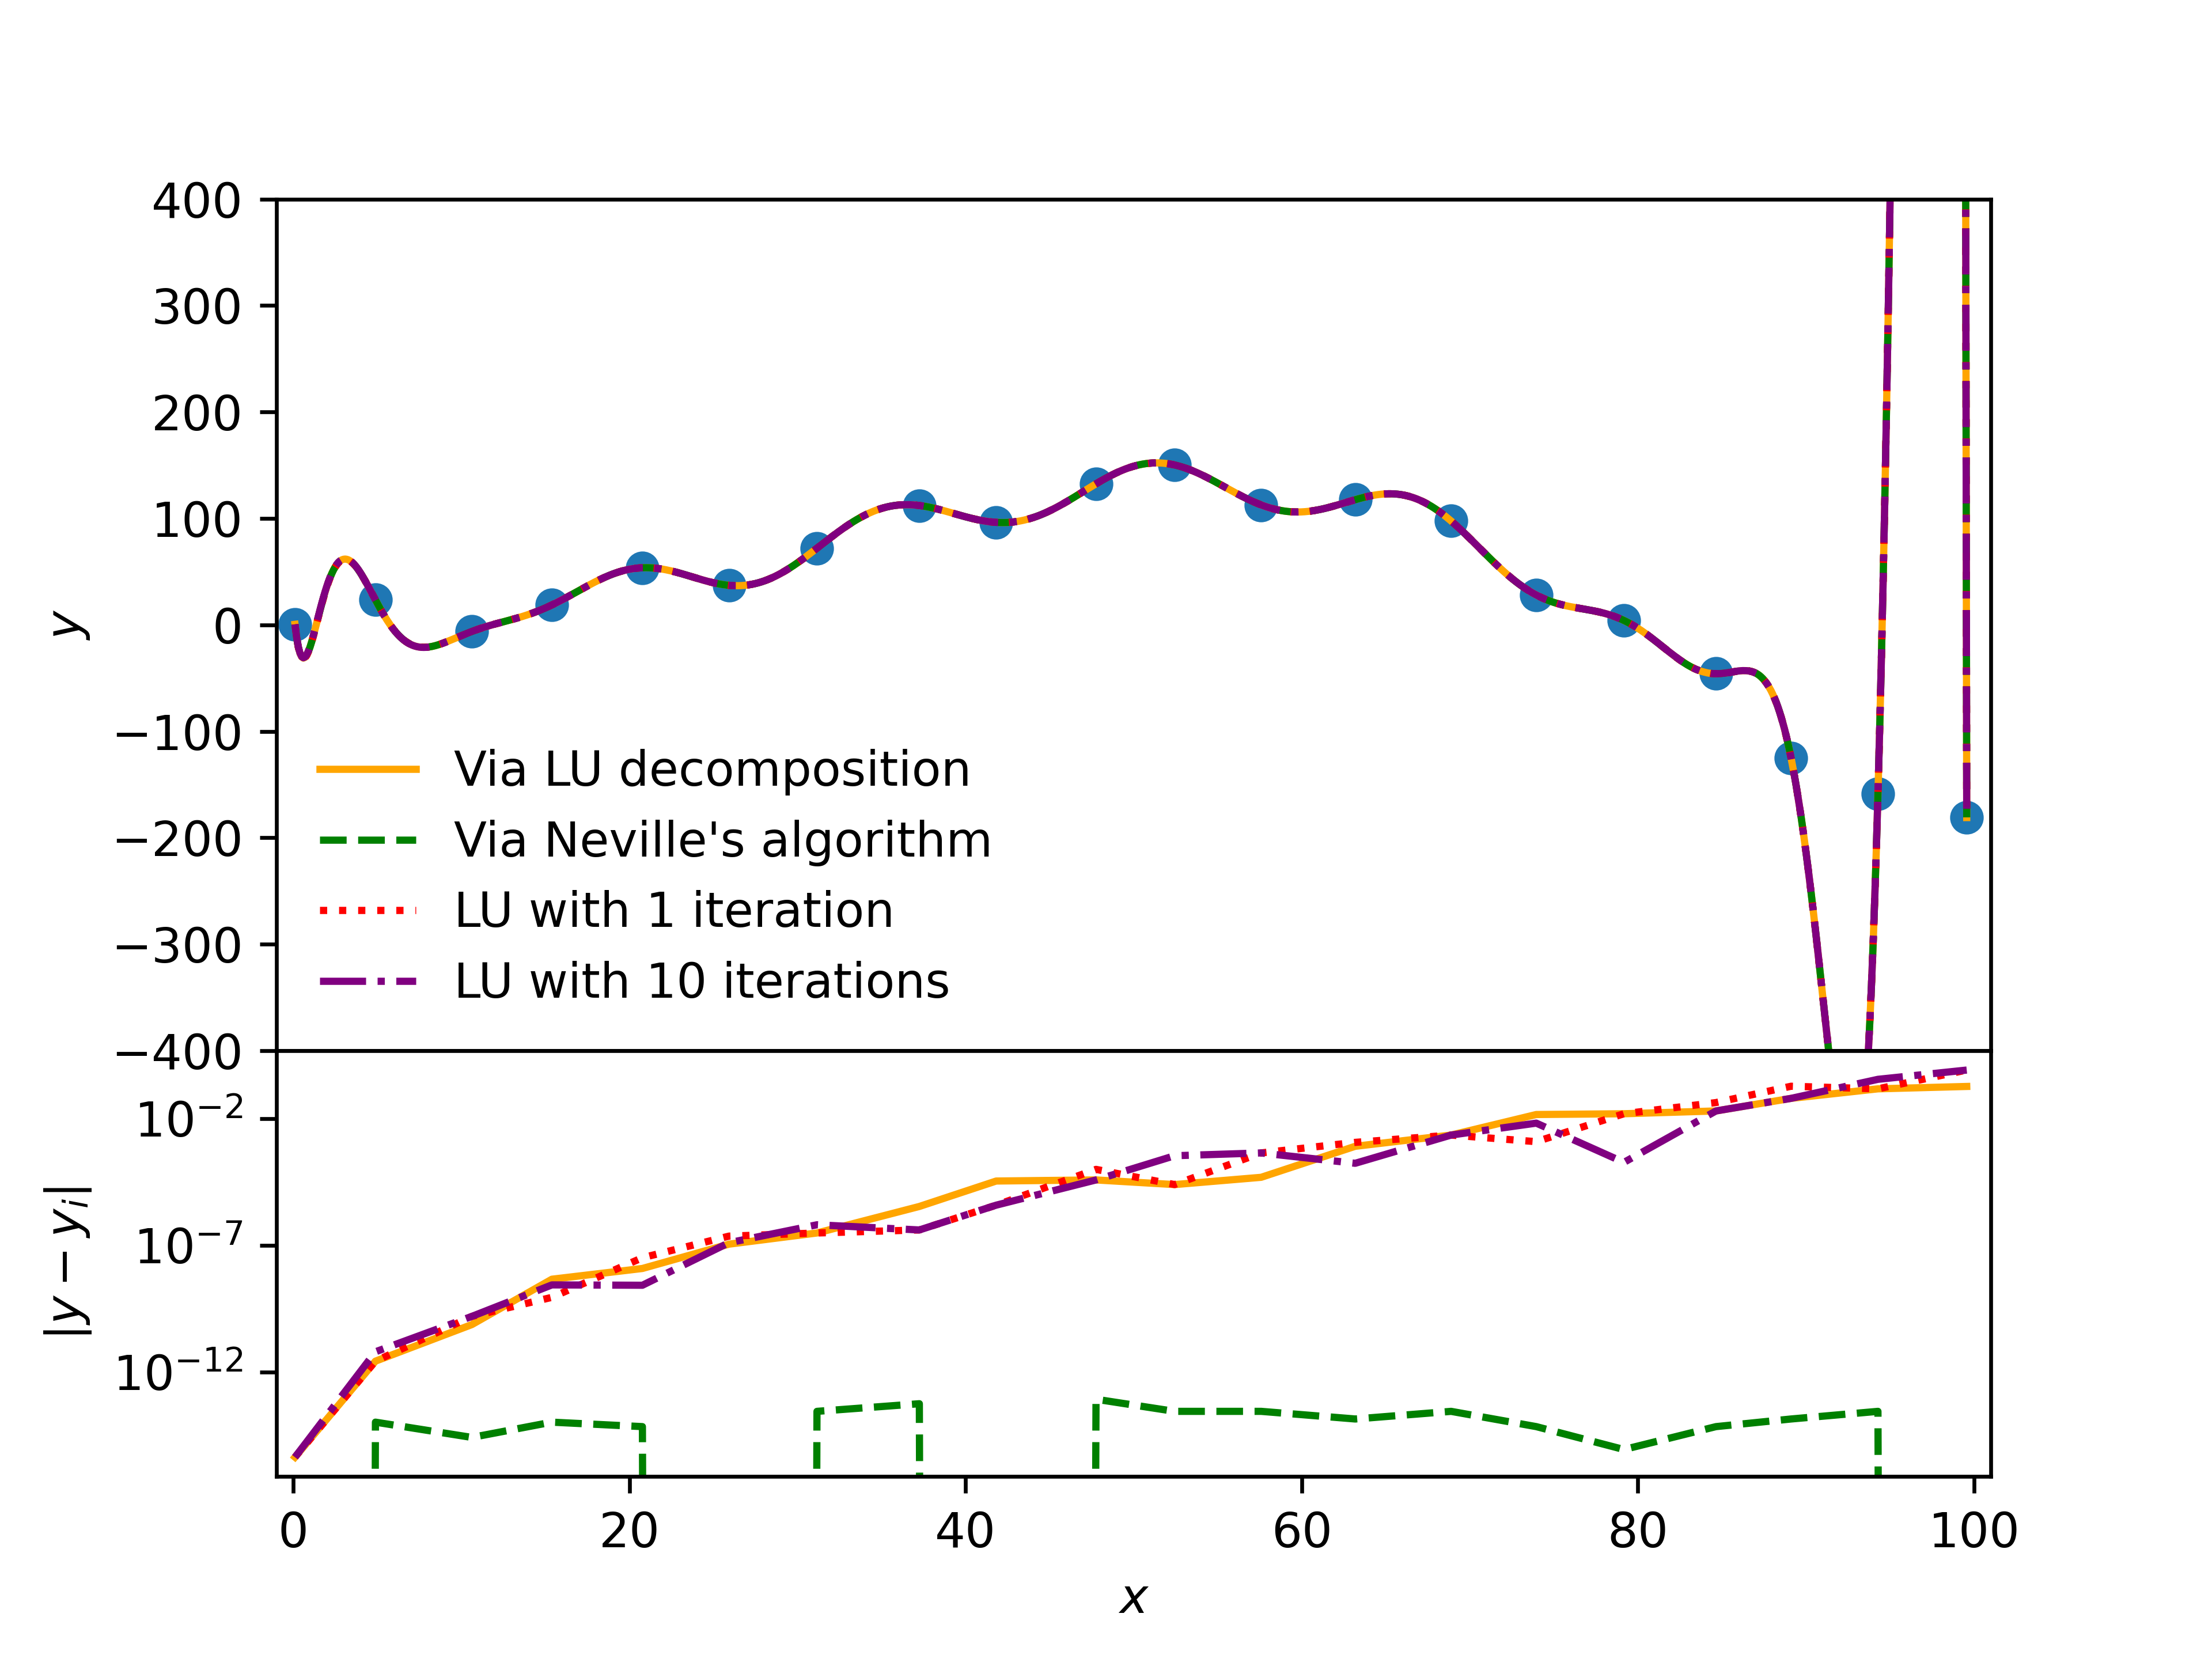
\includegraphics[width=\textwidth]{plots/my_vandermonde_sol_2c.png}
    \caption{Top panel: The provided data is overplotted with the unique polynomial that goes through all points, calculated with different methods.
    Bottom panel: The absolute error of the solving methods. A perfect solution would exactly pass through all points. This allows us to assess the accuracy 
    each algorithm.
    } \label{fig:vdmonde}
\end{figure}

As seen in Fig. 1, the interpolation method yields the most accurate result. This may be expected, because the Vandermonde matrix 
involves the computation of high powers of numbers. This may amplify errors and cause numerical instability due to the combination of very large
and very small numbers in the Vandermonde matrix. The latter results in a very high condition number, meaning the matrix is (close to) ill-conditioned.
The error increases for larger x using the LU decomposition, because here these high powers have more influence on the solution.

In contrast, Neville's algorithm gives a lower error at the data points, because it uses these data points explicitly as inputs for the iterative polynomials
it works with, whereas the LU-decomposition method only uses the data points in the form of a Vandermonde matrix, which leaves more room for error accumulation
at these points.

Iterating on the original solution does not seem to give a more accurate result. This means we are already at the best possible accuracy.

Finally, we compare the runtime of each method with the \texttt{timeit} module. The LU decomposition method
is on the order of a few 100 times faster than the polynomial interpolation method. This may be expected,
because Neville's algorithm involves a lot more computations (bisection, looping over polynomials, etc.) 
than the LU decomposition method. This is the cost of the improved accuracy. This makes interpolation
a less viable method for large datasets.

Calculating 10 iterative improvements takes about 4-5 times longer than calculating the solution a single time.
I would have expected this to be a bit more than 10 times longer, because for-loop computation time scales 
linearly with the number of loops.

\noindent The code:

\lstinputlisting{timing.py}

\noindent The output:

\input{timing_output.txt}
